\documentclass[12pt]{beamer}
\usepackage{beamerthemeHannover, graphicx, clrscode, amsmath, amssymb, multicol}
\usepackage{verbatim}
\setbeamercolor{sidebar}{use=structure,bg=gray!60!green}
\title{Mimosa \\ \small{ Miniature Model Organism Sequence Aligner } }
\author[Leto]{Jonathan "Duke" Leto \\ Sol Genomics Network \\ http://solgenomics.net }
\date{}

\begin{document}

\frame{
    \titlepage
    \begin{center}
    \end{center}
}

\frame{
    \frametitle{What is Mimosa?}
    \begin{center}
        \begin{itemize}
            \item Next Generation of the SGN BLAST Tool
            \item Why does everyone reinvent the web alignment wheel?
            \item Why are they all square-ish ?
        \end{itemize}
    \end{center}
}

\frame{
    \frametitle{Design Goals}
    \begin{center}
        \begin{itemize}
            \item Pluggable
            \item User-Friendly
            \item Interoperable
            \item Easy To Deploy
        \end{itemize}
   \end{center}
}
\frame{
    \frametitle{Pluggability}
    \begin{center}
        \begin{itemize}
            \item Supports any database that DBI knows about
            \begin{itemize}
                \item SQLite
                \item PostgreSQL
                \item MySQL
                \item ...
            \end{itemize}
            \item Can run standalone or through webserver
        \end{itemize}
    \end{center}
}

\frame{
    \frametitle{User-Friendly}
    \begin{center}
        \begin{itemize}
            \item Tooltipped context-sensitive help
            \item Support different workflows for different user types
            \item Download all results in various formats
            \item Ability to save user preferences
            \begin{itemize}
                \item Preferred Organism
                \item Default e-value/substitution matrix/etc
            \end{itemize}
        \end{itemize}
    \end{center}
}

\frame{
    \frametitle{Easy To Deploy}
    \begin{center}
        \begin{itemize}
            \item What, you don't want to install 5000 CPAN modules?
            \item Packages will be available for Debian/Ubuntu/etc
            \item Goal: Download 1 file, Run 1 command to install
        \end{itemize}
    \end{center}
}

\frame{
    \frametitle{Interoperable}
    \begin{center}
        \begin{itemize}
            \item Work with current GMOD software
            \item Web API to integrate with other web services
            \item Possibly an Intermine Plugin?
        \end{itemize}
    \end{center}
}

\frame{
    \frametitle{Screenshot}
    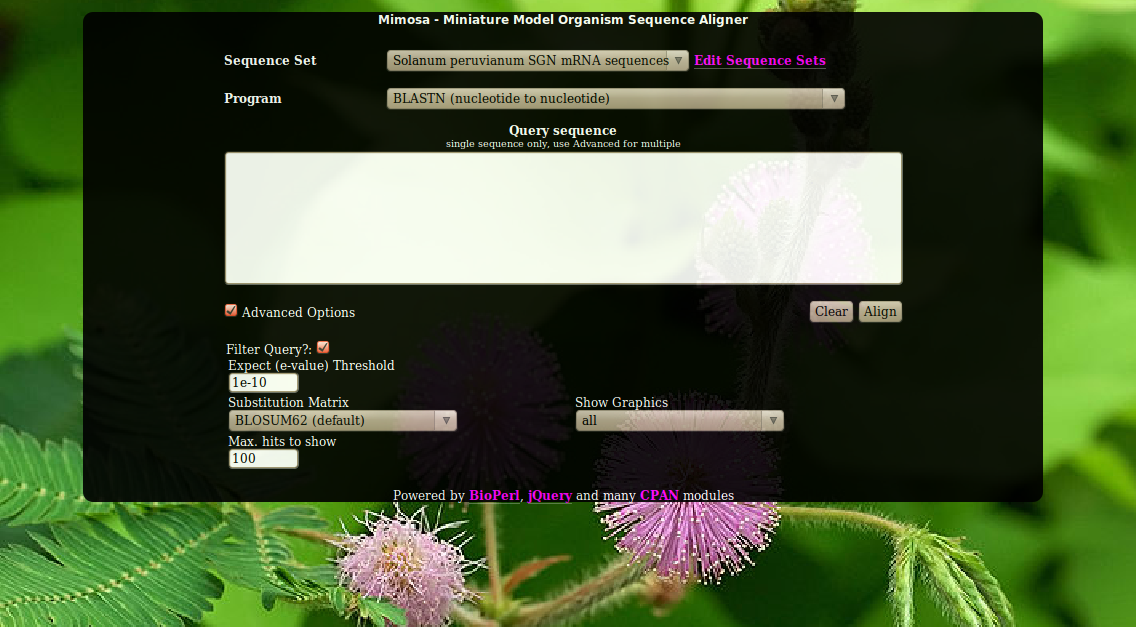
\includegraphics[width=10.5cm, height=9.5cm]{mimosa_new}
}

\frame{
    \frametitle{Killer Features}
    \begin{itemize}
        \item Web-based Sequence Set Administration
        \item Sequence Set Filtering by Organism
        \item Automated Sequence Set Updates (from NCBI/etc)
        \item What else?
    \end{itemize}
}

\frame{
    \frametitle{What is under the hood?}
    \begin{itemize}
        \item Moose
        \item BioPerl
        \item Bio::Chado::Schema
        \item Mason
        \item jQuery
    \end{itemize}
}

\frame{
    \frametitle{ Thanks }
    \begin{itemize}
        \item Boyce Thompson Institue for Plant Research
        \item NESCent
    \end{itemize}
}

\frame{
    \frametitle{ Resources }
    \begin{center}
        \begin{itemize}
           \item http://github.com/GMOD/mimosa
           \item http://solgenomics.net
           \item \#gmod on irc.freenode.net
        \end{itemize}
    \end{center}
}
\end{document}
